\documentclass[xcolor=dvipsnames]{beamer}
\usepackage{xcolor}
\usepackage{graphicx}
\usepackage{xmpmulti}

% \usetheme{Antibes}
\usetheme{boxes}
\usecolortheme{wolverine}

\setbeamercolor{emph}{fg=orange}
\renewcommand<>{\emph}[1]{%
  {\usebeamercolor[fg]{emph}\only#2{\itshape}#1}%
}

\title{Product Structure Theorems}
\author{}
\date{}
\institute{
  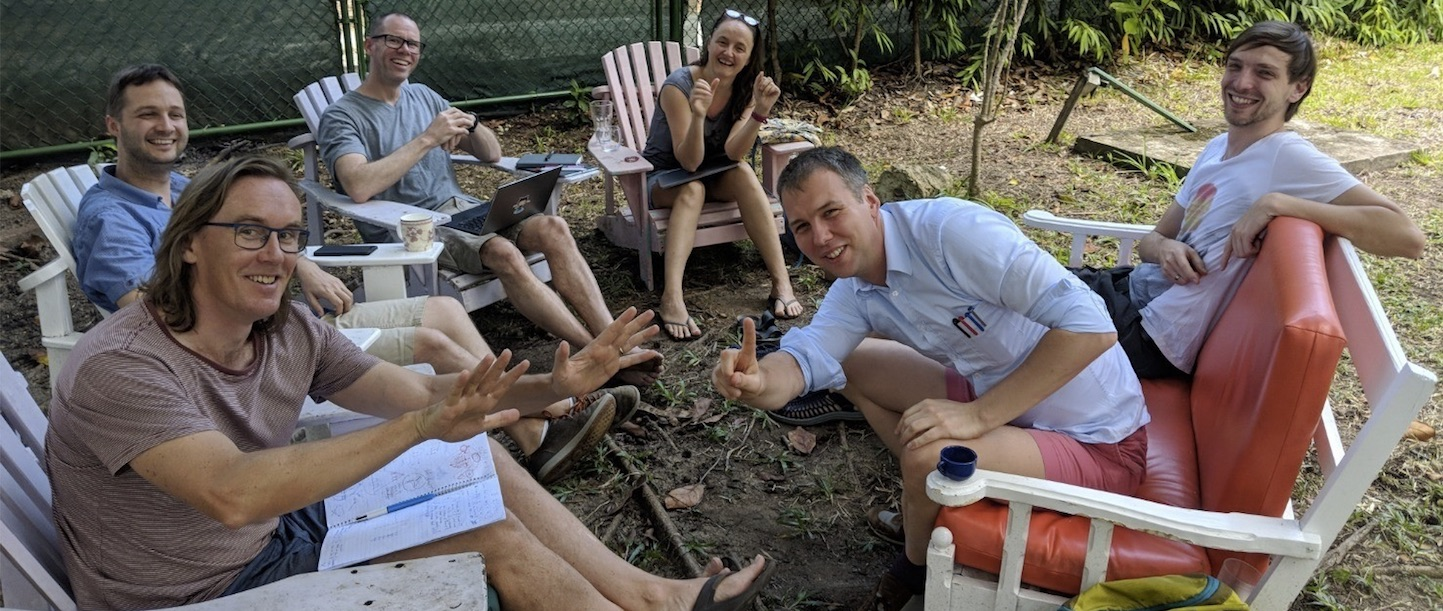
\includegraphics[width=.6\textwidth]{images/Queue11} \\
  $G\subseteq H\boxtimes P$ \\
  % \resizebox{.3\textwidth}{
  % \includegraphics[scale=.55]{figs/planar-subgraph}\raisebox{.077\textwidth}{$\subseteq$}\includegraphics[scale=.55]{figs/product-lhs}
  % }
}

\DeclareMathOperator{\tw}{tw}

\newcommand{\colored}[2]{{\color{#1}#2}}


\begin{document}
\maketitle

\begin{frame}
  \frametitle{Outline}

  \begin{itemize}
    \item Theorem Statement
    \item Motivation
    \item The Product Structure Theorem for planar graphs
    % \item Proof sketch
    \item Generalizations and variants
    \item Applications
  \end{itemize}
\end{frame}

\begin{frame}
  \frametitle{Ranking Graph Classes by Complexity}

  \colored{ForestGreen}{Simple}
  \begin{itemize}
    \item Paths (forests of paths)
    \item Trees (forests)
    \item $k$-Trees (graphs of treewidth at most $k$)
    \item $\vdots$
    \item Planar graphs
    \item $\vdots$
    \item All graphs
  \end{itemize}
  \colored{red}{Complicated}

  % \includegraphics{figs/product-lhs}
  % \includegraphics[scale=.5]{figs/planar-subgraph} \raisebox{.11\textwidth}{$\subseteq$}%
  % \only<1>{\includegraphics{figs/product-rhs}}%

\end{frame}


\begin{frame}
  \frametitle{Informally}

  \begin{itemize}[<+->]
    \item Can we \emph{factor} a planar graph into simpler graphs?
    \item Yes! Every planar graph is contained in the \emph{strong product} of a graph $H$ of \emph{treewidth} at most $8$ and a \emph{path} $P$ \\ ($G\subseteq H\boxtimes P$)
  \end{itemize}
  \includegraphics{figs/planar-subgraph}%
  \only<4>{\raisebox{.11\textwidth}{$\subseteq$}\includegraphics{figs/product-rhs}}%
  \only<3>{\raisebox{.11\textwidth}{$\subseteq$}\includegraphics{figs/product-lhs}}
\end{frame}

\begin{frame}
  \frametitle{Treewidth}

  A \emph{tree-decomposition} of a graph $G$ represents each vertex as a subtree of a
  tree $T$ so  that the subtrees of adjacent vertices intersect in
  $T$\\[2ex]
  \begin{minipage}{.3\textwidth}
  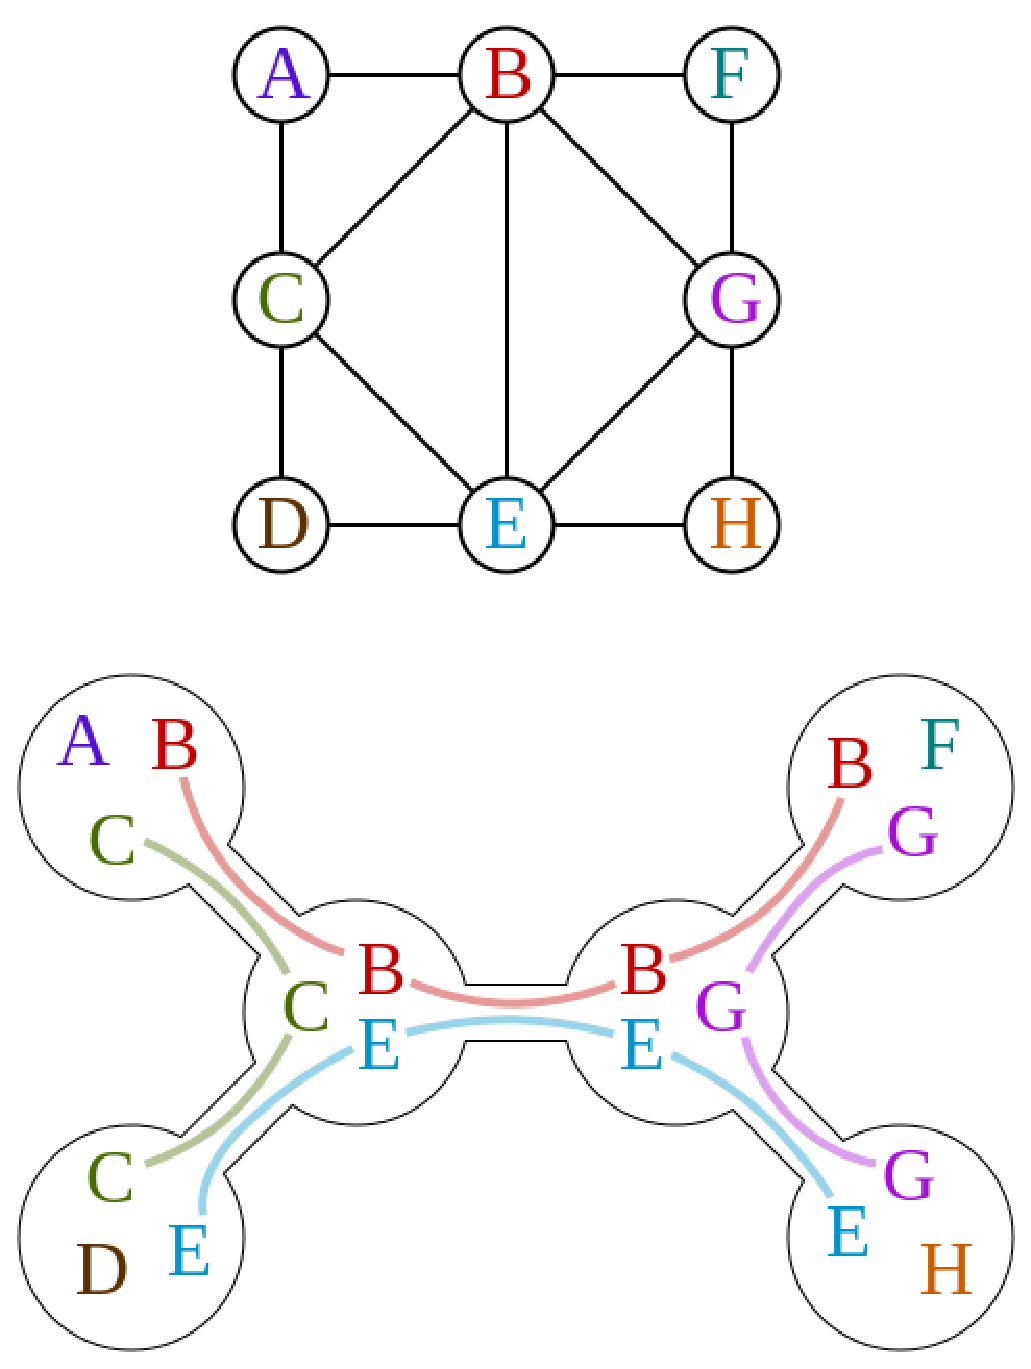
\includegraphics[height=.5\textheight]{images/treedecexam}
  \end{minipage}%
  % \only<2->{
    \begin{minipage}{.69\textwidth}
      % \bigskip\bigskip
      \vspace{-5em}
      \emph{width}  $:=$ maximum bag size ${}-1$ \\[1em]
       % \bigskip
      \emph{treewidth} $:=$ min width of tree-decomposition of $G$
    \end{minipage}
  % }
  \vfill\hfill{\tiny\textcolor{gray}{ [Images courtesy of Wikipedia]}}
\end{frame}

\begin{frame}
  \frametitle{The Strong Graph Product $\boxtimes$}
  \begin{itemize}
      \item[] For two graphs $A$ and $B$, the \emph{strong product} $A\boxtimes B$ is a graph:
      \begin{itemize}
          \item $V(A\boxtimes B):=V(A)\times V(B)$
          \item $(a_1,b_1)$ and $(a_2,b_2)$ are adjacent if and only if:
          \begin{itemize}
              \item $a_1=a_2$ and $b_1b_2\in E(B)$;
              \item $a_1a_2 \in E(A)$ and $b_1=b_2$; or
              \item  $a_1a_2 \in E(A)$ and $b_1b_2 \in E(B)$.
          \end{itemize}
      \end{itemize}
  \end{itemize}
  \begin{center}
      \includegraphics{figs/product-lhs} \raisebox{.11\textwidth}{$=$} \includegraphics{figs/product-rhs}
  \end{center}
\end{frame}

\begin{frame}
  \frametitle{The Product Structure Theorem for Planar Graphs}

  \textbf{Theorem (Dujmović-Joret-Micek-M-Ueckerdt-Wood 2019):} For every planar graph $G$, there exists a planar graph $H$ of treewidth at most $8$ and a path $P$ such that $G$ is a subgraph of $H\boxtimes P$.

  \includegraphics{figs/planar-subgraph}%
  % \only<4>{\raisebox{.11\textwidth}{$\subseteq$}\includegraphics{figs/product-rhs}}%
  \raisebox{.11\textwidth}{$\subseteq$}\includegraphics{figs/product-lhs}
\end{frame}

\begin{frame}
  \frametitle{Why?}

  $G\subseteq H\boxtimes P$
  \begin{itemize}[<+->]
    \item $H$ is a graph of treewidth at most $8$
    \item Many problems are easy for $H$
    \item Extending a solution from $H$ to $H\boxtimes P$ is sometimes easy
    \item Examples:
    \begin{itemize}
      \item queue number
      \item nonrepetitive colouring
      \item $p$-centered colouring
      \item $\ell$-vertex ranking
      \item adjacency labelling (universal graphs)
    \end{itemize}
  \end{itemize}
  \begin{center}
    \resizebox{.5\textwidth}{!}{
      \includegraphics{figs/planar-subgraph}%
      \raisebox{.11\textwidth}{$\subseteq$}\includegraphics{figs/product-lhs}
    }
  \end{center}
\end{frame}

\begin{frame}
  \frametitle{The Precursor}

  \textbf{Theorem (Siebertz-Pilipczuk 2018):}  For any planar triangulation $G$, there exists a partition $\mathcal{P}$ of $V(G)$ such that
  \begin{itemize}
    \item<2-> Each part of $P$ induces a \emph{geodesic} (shortest path) in $G$; and
    \item<3-> The quotient graph $H:=G/\mathcal{P}$ has treewidth at most $8$
  \end{itemize}

  \begin{center}
    \only<1>{\includegraphics[width=.8\textwidth]{figs/lhp-1}}%
    \only<2>{\includegraphics[width=.8\textwidth]{figs/lhp-2}}%
    \only<3->{\includegraphics[width=.8\textwidth]{figs/lhp-3}}%
    % \only<4->{\includegraphics[width=.8\textwidth]{figs/lhp-4}}%
    % \only<5>{\includegraphics{figs/lhp-5}}%
  \end{center}
\end{frame}

\begin{frame}
  \frametitle{Layered $H$-Partitions}
  \onslide<+->{
  \textbf{Theorem (Dujmović-Joret-Micek-M-Ueckerdt-Wood 2019):} For any planar triangulation $G$ and any \emph{breadth-first spanning-tree} $T$ of $G$, there exists a partition $\mathcal{P}$ of $V(G)$ such that
  \begin{itemize}[<+->]
    \item Each part of $P$ induces a \emph{vertical path} in $T$
    \item The quotient graph $H:=G/\mathcal{P}$ has treewidth at most $8$
  \end{itemize}
  }
  \begin{center}
    \only<1>{\includegraphics[width=.8\textwidth]{figs/lhp-4}}%
    \only<2>{\includegraphics[width=.8\textwidth]{figs/lhp-5}}%
    \only<3->{\includegraphics[width=.8\textwidth]{figs/lhp-6}}%
    % \only<4->{\includegraphics[width=.8\textwidth]{figs/lhp-4}}%
    % \only<5>{\includegraphics{figs/lhp-5}}%
  \end{center}
\end{frame}


\begin{frame}
  \frametitle{Equivalence}

  Layered $H$-partition theorem and product structure theorem are equivalent:
  \begin{center}
    \multiinclude[<+>][format=pdf,start=1]{figs/comparison}
  \end{center}
\end{frame}

\begin{frame}
  \frametitle{Proof of Layered $H$-Partition Theorem}
  \framesubtitle{(Short version: Tutte's Method)}

  \begin{itemize}
      \item Copy the proof of Pilipczuk-Siebertz (2018) except
      \begin{itemize}
          \item<2-> replace ``shortest path in $G$ from $v$ to $C$'' with
          \item<3-> ``shortest path in $T$ from $v$ to $C$''
          \item<4-> check that everything still works
      \end{itemize}
  \end{itemize}
  \begin{center}
    \multiinclude[<+>][format=pdf,start=1]{figs/proof}
  \end{center}
\end{frame}


\begin{frame}
    \frametitle{Second Version}

    \textbf{Theorem (Dujmović-Joret-Micek-M-Ueckerdt-Wood 2019):}
    For every planar graph $G$ there exists a planar graph $H$ of treewidth at most \emph{$3$} such that $G\subseteq H\boxtimes P\boxtimes K_3$.
    \begin{center}
        \includegraphics{figs/hpk3}
    \end{center}
    \onslide<2->{Useful when the (simple) treewidth of $H$ is important \\
      planar and treewidth-$3$ $\Longleftrightarrow$ simple treewidth $3$
    }

\end{frame}

\begin{frame}
    \frametitle{Algorithmic Version}

    \textbf{Theorem (M 2021):}
    There exists an $O(n\log n)$ time algorithm that, given an $n$-vertex planar triangulation $G$ finds $H$ and $P$ and the mapping $V(G)\to V(H\boxtimes P)$.

    \begin{center}
    \includegraphics[scale=.35]{figs/sperner-1}
    \includegraphics[scale=.35]{figs/sperner-2}
    \includegraphics[scale=.35]{figs/sperner-explode-2}
    \end{center}
    \url{https://github.com/patmorin/lhp}
\end{frame}

\begin{frame}
    \frametitle{Generalizations}

    Similar$^*$ product structure theorems for

    \begin{itemize}[<+->]
       \item graphs of bounded genus and apex-minor free graphs (Dujmović-Joret-Micek-M-Ueckerdt-Wood 2019);
       \item bounded degree graphs that exclude a fixed graph as a minor (Dujmović-Esperet-M-Walczak-Wood 2020);
       \item $k$-planar graphs and $(g,k)$-planar graphs (Dujmović-M-Wood 2019).
   \end{itemize}
   \begin{center}
     \onslide<1->{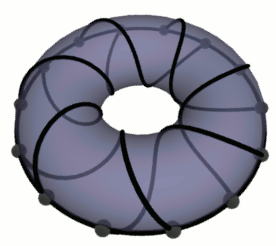
\includegraphics[width=.3\textwidth]{images/Toroidal_graph_sample}}
     \onslide<3->{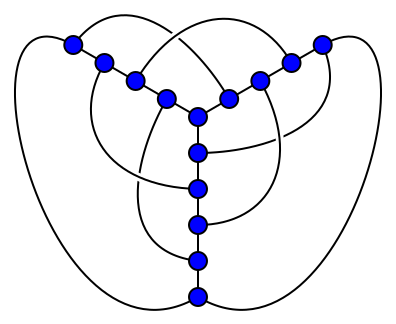
\includegraphics[width=.3\textwidth]{images/3-crossing_Heawood_graph}}
   \end{center}

{\small $^*$$G\subseteq H\boxtimes P$, only the treewidth of $H$ changes}

{\tiny By David Eppstein - Own work, Public Domain, \url{https://commons.wikimedia.org/w/index.php?curid=9852307}}

\end{frame}

\begin{frame}
    \frametitle{Last Slide}

    \textbf{Next: Applications}
    \begin{itemize}
        \item queue number (David Wood)
        \item nonrepetitive colouring (Louis Esperet)
        \item $p$-centered colouring and $\ell$-vertex ranking (Piotr Micek)
        \item universal graphs (Gwenaël Joret) \\[2em]
    \end{itemize}
    \onslide<2->{
    \begin{center}
        {\Huge Thank You!}
    \end{center}
    }
    \textbf{References:}
    {\tiny
    \begin{itemize}
        \item Michał Pilipczuk, Sebastian Siebertz: Polynomial bounds for centered colorings on proper minor-closed graph classes. \textit{SODA 2019}: 1501-1520 [arxiv:1807.03683]

        \item Vida Dujmović, Gwenaël Joret, Piotr Micek, Pat Morin, Torsten Ueckerdt, and David R. Wood. Planar graphs have bounded queue-number.
        \textit{Journal of the ACM}, 67(4):22:1–22:38, 2020.
        [arxiv:1904.04791]

        \item Vida Dujmović, Louis Esperet, Pat Morin, Bartosz Walczak, and David R. Wood. Clustered 3-colouring graphs of bounded degree. \textit{Combinatorics, Probability and Computing}. Accepted in May 2021. [arxiv:2002.11721].

        \item Vida Dujmović, Pat Morin, and David R. Wood. Graph product structure for non-minor-closed classes. [arxiv:1907.05168].

        \item Pat Morin. A fast algorithm for the product structure of planar graphs. Algorithmica, 83(5):1544–1558, 2021. [arxiv:2004.02530]
% [doi:10.1109/FOCS.2019.00056][video][doi:10.1145/3385731].
    \end{itemize}
    }


\end{frame}



\end{document}
